\section{AMR}

In general, the AMR input looks like:

\begin{lstlisting}
  <AMR>
      <ICE>
        <do_Refluxing>        false    </do_Refluxing>
        <orderOfInterpolation>1         </orderOfInterpolation>
        <Refinement_Criteria_Thresholds>
          <Variable name = "press_CC" value = "1e6" matl = "0" />
        </Refinement_Criteria_Thresholds>
      </ICE>
      <MPM>
        <min_grid_level>-1</min_grid_level>
        <max_grid_level>-1</max_grid_level>
      </MPM>
      <useLockStep>true</useLockStep>    
      <Regridder type="BNR">
        <!--to use hierarchical regridder set the type to "Hierarchical", to use the tiled regridder set the type to "Tiled" -->
        <type> BNR </type>

        <!--General Regridder Settings-->
        <max_levels>2</max_levels>
        <cell_refinement_ratio>    [[2,2,1]]</cell_refinement_ratio>
        <cell_stability_dilation>   [2,2,0]   </cell_stability_dilation>
        <cell_regrid_dilation>   [1,1,0]   </cell_regrid_dilation>
        <min_boundary_cells>       [1,1,0]   </min_boundary_cells>
        
        <!--Hierarchical Specific Settings-->
        <lattice_refinement_ratio> [[4,4,1],[2,2,1]]  </lattice_refinement_ratio>
        
        <!--Berger Rigoutsos Specific Settings-->
        <min_patch_size>  [[8,8,1]] </min_patch_size>
        <patch_ratio_to_target>.2</patch_ratio_to_target>

        <!--Tiled Specific Settings-->
        <min_patch_size>  [[8,8,1]] </min_patch_size>
        <patches_per_level_per_proc>8</patches_per_level_per_proc>         
      </Regridder>
    </AMR>

\end{lstlisting}

If you run an ICE simulation, then you must specify the ICE section. 

\begin{itemize}
\item \TT{do_refluxing} - specifies whether or not to perform refluxing,
  which equalizes the face values of coarse/fine boundaries between
  levels.
\item orderOfInterpolation - specifies how many coarse cells to use
  when refining the coarse-fine interface (see below).
\item the \TT{Refinement_Criteria_Thresholds} section specifies the
  variables whose value will determine where to mark refinement flags,
  see below. Variables need only be specified on adaptive problems.
\item \TT{min_grid_level} (optional) - coarsest level to run ICE on
  (default = 0).
\item \TT{max_grid_level} (optional) - finest level to run ICE on (default
  = max-level -1).

\end{itemize}

If you run an MPM simulation, you must specify the MPM section, and
set \TT{min_grid_level} and \TT{max_grid_level} to the finest level of the
simulation, 0-based (i.e., if there are 2 levels, the level needs to
be set to 1). A shortcut to this is to set min- and \TT{max_grid_level} to
-1.

\begin{itemize}
\item useLockStep - Some simulations require a lock step cycle (mpmice
  and implicit ice), as there has to be inter-level communication in
  the middle of a timestep. See "W-cycle" diagram below. Otherwise the
  time refinement ratio will be computed from the cell refinement
  ratio.
\end{itemize}


The presence of the Regridder section specifies you want to run an
adaptive problem.
\begin{itemize}
  \item type (optional) - sets the Regridder type. The options are
   "Tiled", "BNR" (Berger-Rigoutsos), "Hierarchical" (default).
  \red{Only the "Tiled" regridder can be used with ICE, AMRICE, MPMAMRICE problems.}
 \item \TT{max_levels} - maximum number of levels to create in the grid. 
 \item \TT{cell_refinement_ratio} - How much to refine a cell in each
   dimension. This can be specified in a comma-separated list, as in
   the example for \TT{lattice_refinement_ratio}, and for each level not
   included in the list, it will be set to the last value specified.
 \item \TT{cell_stability_dilation} - How much to pad the refinement flags
   in each dimension for stability reasons.
 \item \TT{cell_regrid_dilation} - How much to pad the refinement flags in
   each dimension in order to reduce regridding frequency.
 \item \TT{min_boundary_cells} - The minimum number of cells that needs to
   exist between one level's coarser level and its finer level (i.e.,
   between level 0 and 2).
\end{itemize}

Hierarchical Specific Settings

\begin{itemize}
\item \TT{lattice_refinement_ratio} - Specific to Hierarchical
  Regridder. Determines how many patches to potentially divide a
  coarser patch into on the finer level. See Regridding section below.
\end{itemize}

Berger-Rigoutsos Specific Settings 

\begin{itemize}
\item \TT{min_patch_size} - sets the minimum patch size created by the
  regridder per level. This size must divide evenly into the
  resolution and must be divisible by the cell refinement ratio.
\item \TT{patch_ratio_to_target} - sets the maximum patch size to the
  average work load per processor times this value. Theoretical load
  imbalance should be close to one half of this value. Setting this
  value too small will create an excess number of patches and cause
  excessive overhead. .2 seems to be a reasonable value.
\end{itemize}

Tiled Specific Settings 
\begin{itemize}
\item \TT{min_patch_size} - sets the minimum patch size created by the
  regridder per level. This size must divide evenly into the
  resolution and must be divisible by the cell refinement ratio.
\item \TT{patches_per_level_per_proc} - sets the number of patches per
  level per processor that the load balancer attempts to achieve. If
  the number of patches is significantly more than the number
  specified the tiled regridder will increase the tile size by a
  factor of two in order to reduce the number of patches.
\end{itemize}

If you are using the Berger-Rigoutsos regridder you should also
include a  LoadBalancer~\ref{loadbalancer}.


\subsection{AMR Grids}


There are two ways to run with mesh-refinement, either adaptive or
non-adaptive (static). Adaptive grids are created based on the
existence of refinement flags that are created during the
simulation. A regridder will take the flags, and, wherever there are
refinement flags, patches are constructed around them on a finer
level. See more on Regridding below. Static grids are constructed from
the set of levels in the input file.

\paragraph{Regridding}


For an adaptive problem, specify the Regridder section in the input
file.
 
The Hierarchical regridder works as follows: 

Divide each patch into subpatches according to the
\TT{lattice_refinement_ratio}. E.g., with a ratio of [2,2,2], it will
create 8 subpatches. Then, if there are refinement flags within the
region of that subpatch, then a patch (with resolution increased by
the \TT{cell_refinement_ratio}) will be added with the subpatch's range on
the next finer level. This regridder is inefficient and has been
superseded by the Tiled regridder.

The Berger-Rigoutsos regridder works as follows: 

Tiles of the size of the minimum patch size are laid across the next
finer level. The refinement flags are then used to give each of these
tiles a single flag indicting if a flag exists within them. The
Berger-Rigoutsos algorithm is then used to create an initial patch
set. Next a post processing phase splits patches in order to meet
alignment constraints. Finally another post process phase splits the
largest patches further depending on the \TT{patch_ratio_to_target} input
file specification. The Berger-Rigoutsos regridder should produce
patch sets with a much smaller number of patches than the Hierarchical
Regridder causing less overhead allowing decreasing AMR
overhead. Unfortunately the cost of the running the BNR algorithm can
be substantial at large numbers of processors and the patch sets
produced by this regridder are difficult to load balance. Because of
this the Tiled regridder should be used.

The Tiled regridder works as follows: 

Tiles of the size of the minimum patch size are laid across the next
finer level. Refinement flags are then used to determine which of
those tiles are in the patch set. If the number of tiles is more than
twice the target number of patches then the tiles size is doubled in
the shortest dimension. If the number of tiles is less than the target
number of patches then the tile size is halved in the longest
dimension. The tile size will never get smaller than the minimum
specified tile size. This regridder produces regular patch sets that
are easy to load balance. This regridder will eventually obsolete the
Berger-Rigoutsos and Hierarchical regridders.  The following is some
general regridding information:

If there was a patch on a fine level during one timestep, and then
there are no refinement flags in its region on the coarser level, then
it will be removed during the regridding process.

After patches are added, data are stored on them Then data will be
initialized for those new patches, and the next timestep, those
patches will be included in the regridding process.

A constraint of the Regridder, is that any patch that shares a
boundary with a patch on a different level must be within level. See
(E) and (F) below.

At initialization time, the regridder can be executed and then the
problem reinitialized so the problem can be initialized with all
\TT{max_levels} of refinement.

\begin{figure}[htb]
  \centering
  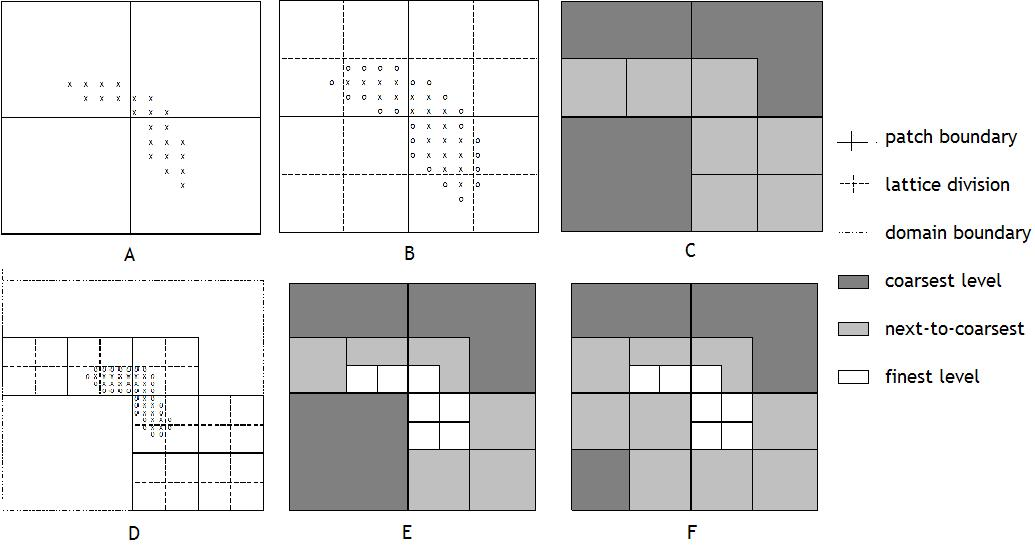
\includegraphics[width=1.\textwidth]{AMR-Regridding.jpg}
  \caption{AMR Regridding}
  \label{fig:amr1}
\end{figure}

n the diagram above, image (A) show 4 coarse patches with some marked
error flags. (B) Shows the subpatches for the next level and has the
error flags dilated. (C) Shows the coarse level together with the fine
level you end up with.

(D) During the next regrid, the next level can create error flags as
well. These are some example error flags that are dilated, with the
subpatches for the next level. (E) shows the reulting level with the
other levels. However there are some patch boundaries that span more
than one level. So (F) we must expand out the middle level to
compensate.

Note that if you you define multiple levels in the input file, all but
the coarsest level will be recycled, and levels will be added where
the Regridder wants to put them.

\paragraph{Static Grids}

Static grids can be defined (but make sure to not include a Regridder
section) in the input file. See the multiple level example in
Grid~\ref{Sec:Grid}.

\subsection{AMR Cycle}

Whether working with an adaptive or a static grid, AMR problems follow
the same cycle. 

In short, there are 3 main AMR operations 
\begin{itemize}

\item Coarsen - This occurs after each execution of a finer level, if
  the time of the finer level lines up with the time of the coarser
  level (see the "W-cycle" diagram). Its data are coarsened to the
  coarser level so that the coarse level has a representation of the
  data at the finest resolution. Also as part of this operation is the
  "reflux" operations, which to makes the fluxes across the face of
  the coarse-fine boundary consistent across levels.
\item Refine the coarse-fine interface - This occurs after the
  execution of each level and after an associated coarsen (if
  applicable). The cells of the boundary of the finer level are
  interpolated with the nearest cells on the coarser level (so the
  finer level stays in sync with the coarser levels).
\item Refine - This occurs for new patches created by the regrid
  operation. Variables that are necesary will be created on those
  patches by interpolation from the coarser level. 
\end{itemize}

After an entire cycle, then we check to see if we need to regrid. If the flags haven't changed such that patches would form, the grid will remain the same. 

In short, these diagrams may be useful: 

"W-cycle" (time refinement ratio of 2) 

\begin{figure}[htb]
  \centering
  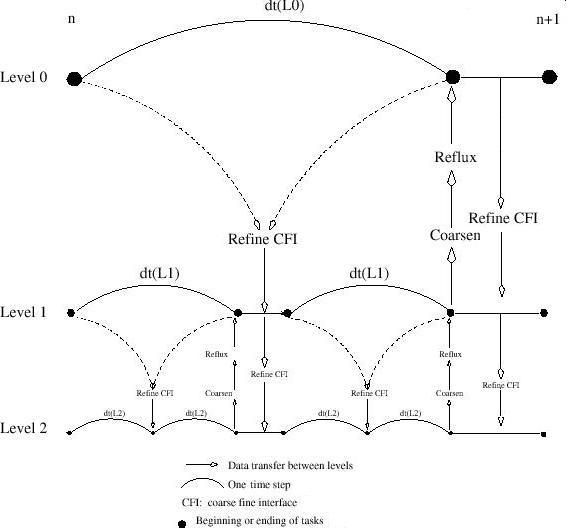
\includegraphics[width=.75\textwidth]{AMR-Cycle-W.jpg}
  \caption{AMR Cycle W}
  \label{fig:amr2}
\end{figure}

``Lockstep cycle''

\begin{figure}[htb]
  \centering
  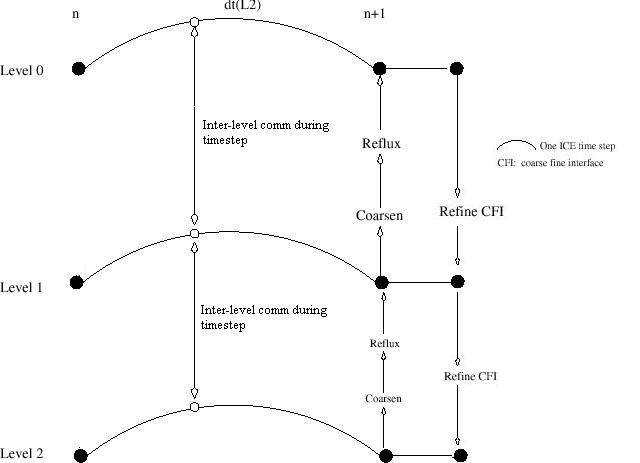
\includegraphics[width=.75\textwidth]{AMR-Cycle-Lock.jpg}
  \caption{AMR Cycle Lock}
  \label{fig:amr3}
\end{figure}
